\documentclass{article}

\usepackage{amsmath} % math stuff
\usepackage{amssymb} % math stuff
\usepackage{array} % equations and stuff
\usepackage{bm} % bold math
%\usepackage{booktabs} % extra table rule options
%\usepackage{caption} % suppressed table numbering; incompatible with revtex, and longtable, I think
\usepackage{comment} % comment environment
%\usepackage{enumitem} % customization of enumeration, itemize, and description
\usepackage[T1]{fontenc} % font encoding for special characters, must also use scalable font package
\usepackage[margin=0.8in]{geometry} % paper sizes and margins (but be careful not to mess up pre-defined pages)
\usepackage{graphicx} % for graphics
%\usepackage{helvet} % default font is the helvetica postscript font
\usepackage[utf8]{inputenc} % special characters in tex input
\usepackage{layouts} % print units like widths
\usepackage{lipsum} % lorem ipsum filler text
\usepackage{lmodern} % scalable font?
\usepackage{longtable} % multi-page tables
\usepackage{makecell} % specify line-breaks in table cells
\usepackage{mathrsfs} % math script font
\usepackage{mhchem} % easier chemical formula
\usepackage{microtype} % allows disabling of ligatures
\usepackage{multicol} % multicolumns
%\usepackage{newcent} % new century schoolbook font
\usepackage{nicefrac}
\usepackage{numprint} % print and format (large) numbers
\usepackage{parskip} % removes paragraph indentation, and adjusts paragraph skip, as well as list items
\usepackage{pdfpages} % add pdf files as pages
%\usepackage{setspace} % adjust text spacing and indents
\usepackage{siunitx} % decimal alignment, and degree symbol
\usepackage{subfigure} % divided figures
%\usepackage{tabu} % extra table options
\usepackage{textcomp} % symbols
\usepackage{threeparttablex} % better footnotes with longtable
\usepackage{titling} % title placement
\usepackage{ulem} % strikethrough text
\usepackage{upgreek} % upright Greek letters
%\usepackage{url} % superceded by hyperref
\usepackage{verbatim} % verbatim environment
\usepackage{xcolor} % colors and color boxes
\usepackage{xspace} % commands that don't eat up white space
\usepackage{hyperref} % links and page setup; should always come last

\hypersetup{
 bookmarks=true,
 colorlinks=true,
 citecolor=blue,
 linkcolor=blue,
 urlcolor=blue,
 pdfstartview={XYZ null null 1.0} % default open view is 100%
}

\DisableLigatures[f,t]{encoding = T1} % disable ff, fi, fl, tt ligatures; without options, it also disables -- = endash
\renewcommand{\arraystretch}{1.0} % extra vertical (and horizontal?) space in tables

% define centered, left- and right-aligned columns with specified widths
\newcommand{\PreserveBackslash}[1]{\let\temp=\\#1\let\\=\temp}
\newcolumntype{C}[1]{>{\PreserveBackslash\centering}p{#1}}
\newcolumntype{L}[1]{>{\PreserveBackslash\raggedright}p{#1}}
\newcolumntype{R}[1]{>{\PreserveBackslash\raggedleft}p{#1}}

\begin{document}

\pagestyle{empty} % don't number pages

% custom title
\begin{center}
{\LARGE Classic Riddler}

\vspace{0.15in}

{\Large 21 January 2022}
\end{center}


\section*{Riddle:}

Rumor has it that readers of The Riddler Ellora Sarkar and Daniel Gomez are getting married this weekend.
Congratulations to you both!
In keeping with the hexagonal design of your wedding backdrop, I thought you might enjoy the following puzzle.
(Riddler Nation, this one's for you, too!)

The larger regular hexagon in the diagram below has a side length of 1.

\vspace{0.1in}
\begin{center}

\includegraphics[width=2.5in]{hexagon1.png}
\end{center}
\vspace{0.1in}

What is the side length of the smaller regular hexagon?

\textit{Extra credit:} If you look very closely, there are two more, even smaller hexagons on top.
Can you see them?
No?
Maybe this animation will help:

\vspace{0.1in}
\begin{center}

\includegraphics[width=2.5in]{hexagon2.png}
\end{center}
\vspace{0.1in}

What are the side lengths of these two even smaller hexagons?

\section*{Solution:}

Although it is not stated, I am assuming that the smaller hexagon is tangent to the larger hexagon, the larger hexagon's vertices lie on the circle, and the smaller hexagon's top two vertices lie on the circle.
With this more complete description, I have drawn a diagram with some points labeled.
C is at the center of the circle (and the larger hexagon), and B is at the center of the smaller hexagon.
In a regular hexagon, the side length is equal to the distance from the center to any vertex.
Thus, if $x$ is the length of $\overline{\mathrm{AB}}$, then $x$ is also the side length of the smaller hexagon.

\vspace{0.1in}
\begin{center}
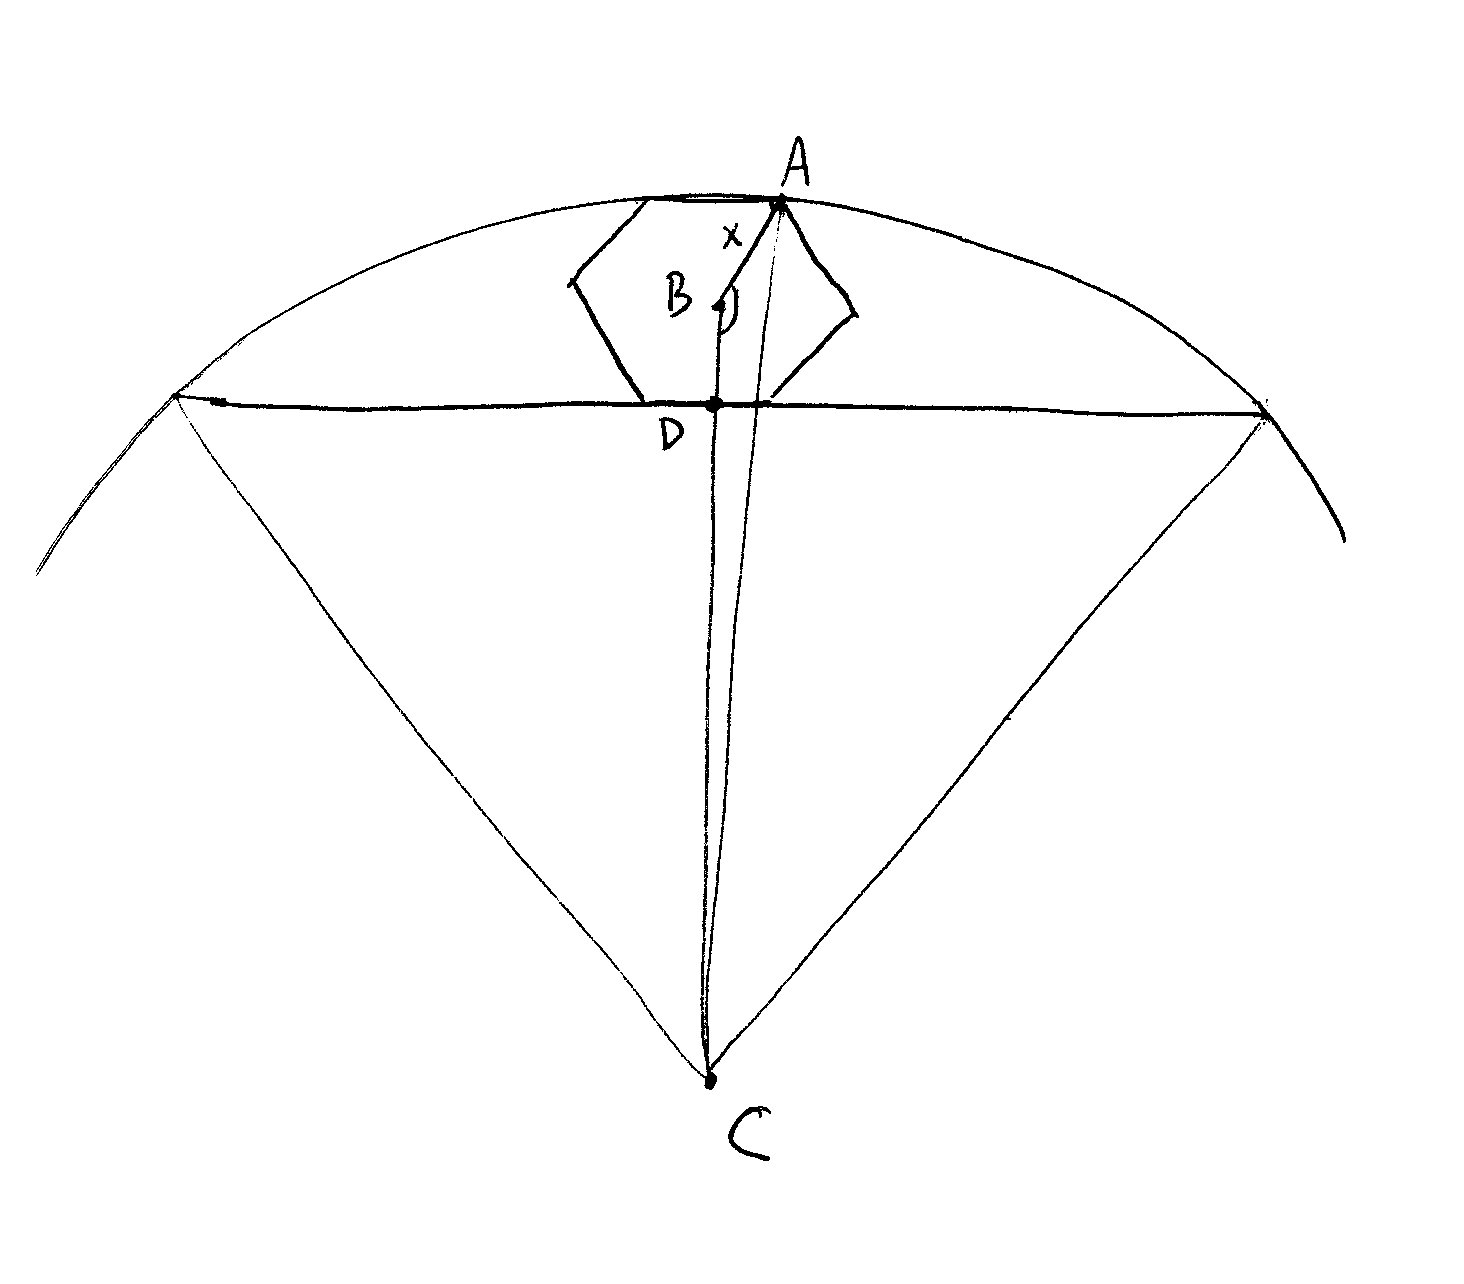
\includegraphics[width=4in]{drawing.jpg}
\end{center}
\vspace{0.1in}

In the diagram, $\overline{\mathrm{AB}}$ is equal to 1.
$\overline{\mathrm{CD}}$ is the altitude of a equilateral triangle of side length 1, which is $\nicefrac{\sqrt{3}}{2}$.
Similarly, $\overline{\mathrm{BD}}$ is $(\nicefrac{\sqrt{3}}{2})x$.
The value of $x$ can be solved using the law of cosines with the triangle $\triangle\mathrm{ABC}$:

\[
1^2 = \left(\frac{\sqrt{3}}{2}+\frac{\sqrt{3}}{2}x\right)^2 + (x)^2 - 2\left(\frac{\sqrt{3}}{2}+\frac{\sqrt{3}}{2}x\right)(x)\cos(\SI{150}{\degree})
\]

Solving this equation conveniently leads to the exact solution \fcolorbox{red}{white}{\textbf{\nicefrac{1}{13}}}\,.

\end{document}